\subsection{Raspberry PI}
\label{sec:raspberry_pi}

Raspberry PIs sind eine Familie an [\acs{SBC}], die von der Raspberry PI Foundation entwickelt und verkauft werden. Die \ac{Arm} basierten Computer haben etwa die Grundfläche einer Kreditkarte und sind etwa 2 cm hoch. Trotz ihrer kleinen Größe haben sie eine achtbare Rechenkapazität (neuere Modelle sogar bis zu 8 GB \ac{RAM} \citev{raspberry_pi_4b}). Dank der vielen Peripheriegeräte, wie \ac{GPIO}, \ac{SPI} und \ac{I2C} sind diese kleinen Computer ideal für das Steuern von Hardware und \ac{IoT} Anwendungen.

\begin{figure}[H]
  \centering
  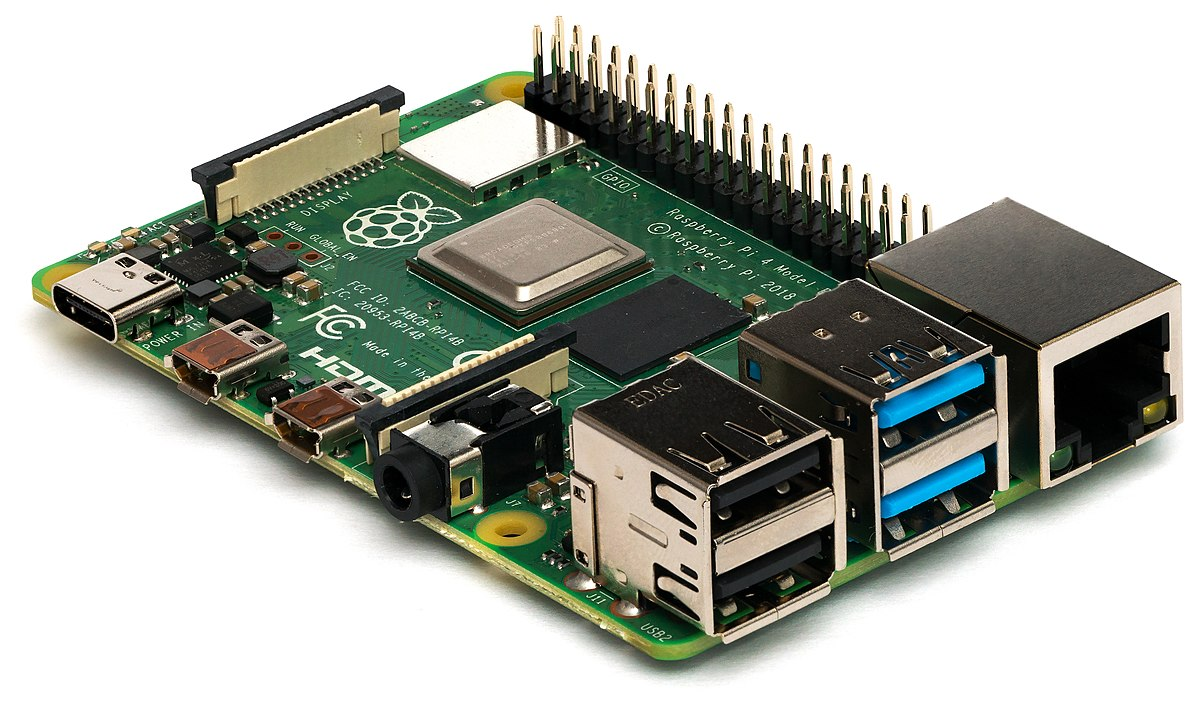
\includegraphics[width=0.75\textwidth]{images/raspberry_pi_4b}
  \caption{Raspberry PI 4b \citev{raspberry_pi_4b}}
  \label{fig:raspberry_pi_4b}
\end{figure}

Anders als bei Mikrocontrollern muss sich der Entwickelnde bei einem Raspberry PI nicht um alles kümmern. Zwischen Hard- und Software gibt es einen [Kernel] und das Linux Betriebssystem. Diese übernehmen viele der Aufgaben und erleichtern die Entwicklung. Somit ist es zum Beispiel möglich eine Python Applikation auf dem Raspberry PI auszuführen.
